\documentclass[english]{scrartcl}
\usepackage[T1]{fontenc}
\usepackage[utf8]{inputenc}
\usepackage[scaled=.8]{beramono}
\usepackage{geometry}
\geometry{verbose,tmargin=3cm,bmargin=3cm,lmargin=3cm,rmargin=3cm}
\usepackage{microtype}
\usepackage[parfill]{parskip}
\usepackage{amsmath}
\usepackage{graphicx}
\usepackage{hyperref}
\usepackage{nameref}
\usepackage{float}
\usepackage{listings}
\usepackage{color}
\usepackage{fancyhdr}
\usepackage{blindtext}

\pagestyle{fancy}
\fancyhf{}
\rhead{Sonja Biedermann 1402891}
\lhead{BUSII}
\cfoot{\thepage}

\newcommand*{\fullref}[1]{\hyperref[{#1}]{\autoref*{#1}~\nameref*{#1}}}

\definecolor{darkgray}{rgb}{0.66, 0.66, 0.66}
\definecolor{asparagus}{rgb}{0.53, 0.66, 0.42}

\lstdefinestyle{s}{
  commentstyle=\color{darkgray},
  keywordstyle=\bfseries,
  morekeywords={},
  stringstyle=\color{asparagus},
  basicstyle=\ttfamily\footnotesize,
  breakatwhitespace=false,
  keepspaces=true,
  numbersep=5pt,
  showspaces=false,
  showstringspaces=false,
}

\lstset{style=s}

\begin{document}

\title{BUSII}

\author{Sonja Biedermann,\\01402891}

\maketitle
\tableofcontents

\section{Implementation Progress}

The static functionalities of the dashboard have been partially implemented.
The only main view that is still missing is the 3D scatterplot, but it will soon
follow, as well as the navigational parts, i.e. the tree and the Gantt chart.

The implementation currently consists of the time series charts for load, torque
and axis speeds, an activity chart and a tabbed chart showing tool information and
the feed rate overrides.

Figure~\ref{fig:screen} shows the current state. Everything is still subject to change,
especially the colors.

\begin{figure}[tb]
    \centering
    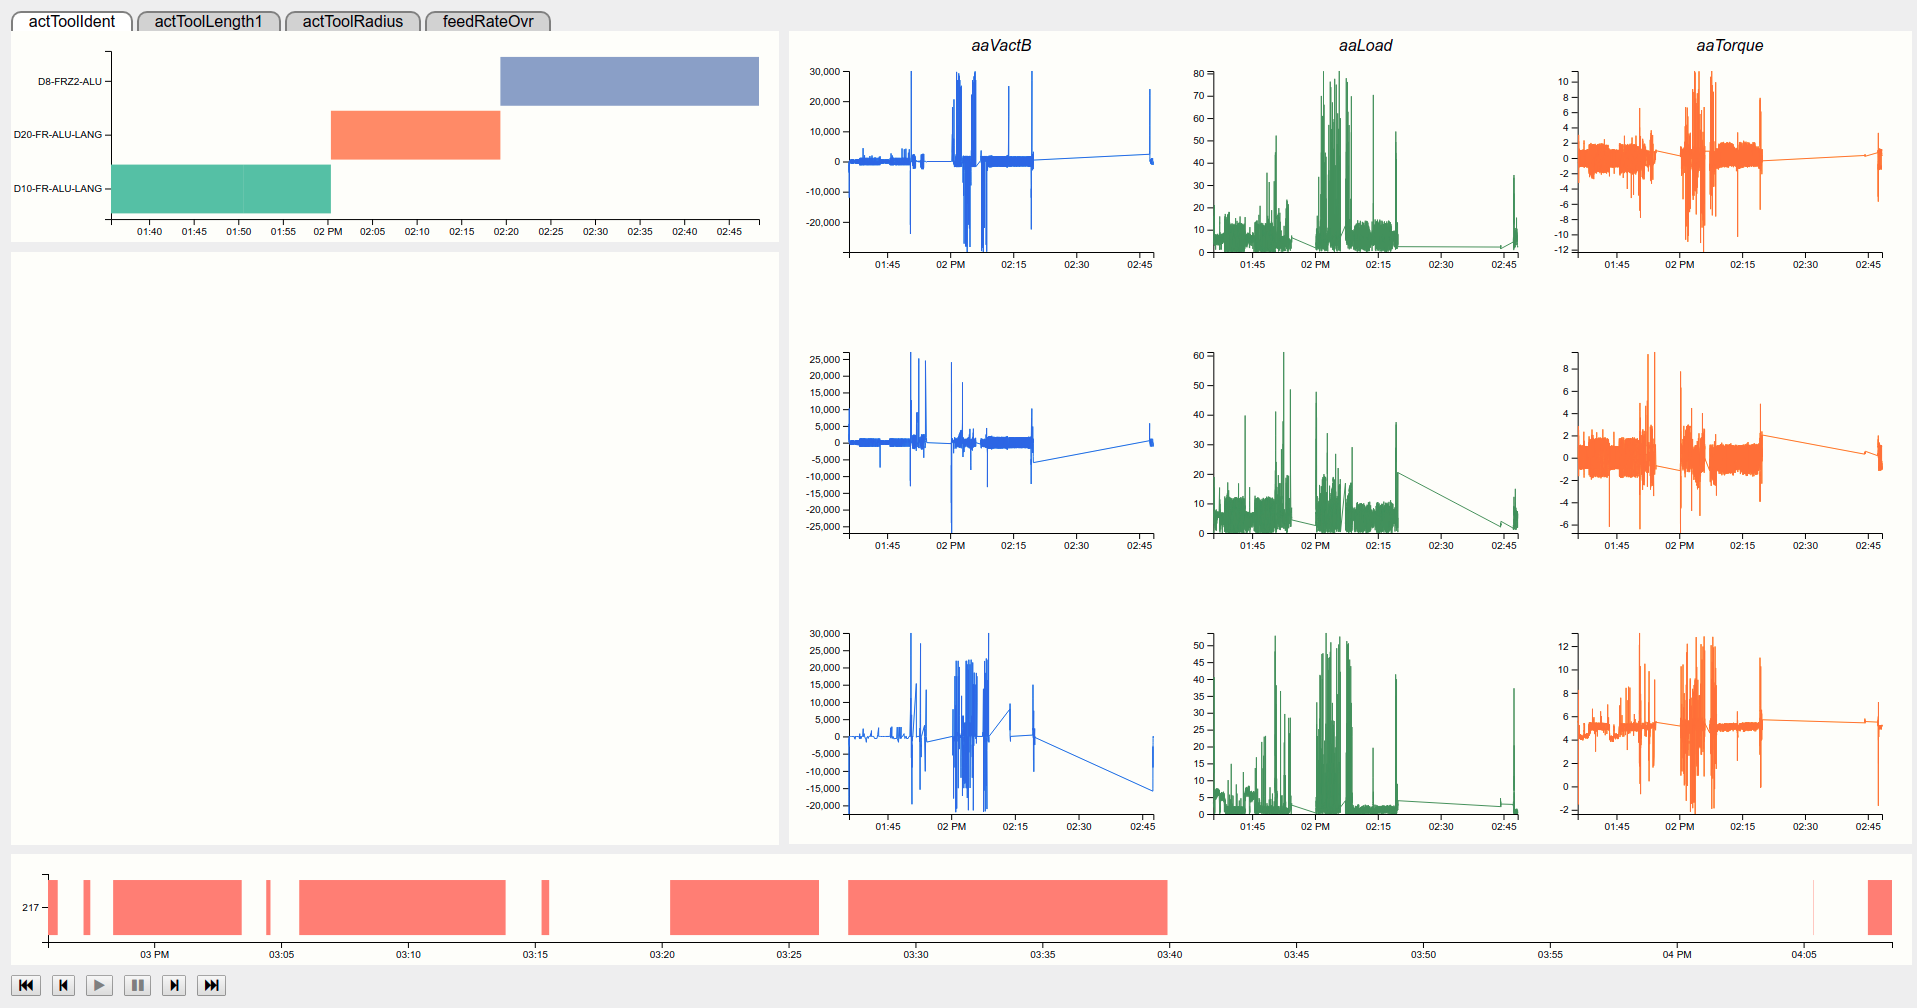
\includegraphics[width=\textwidth]{screen}
    \caption{Screenshot}
    \label{fig:screen}
\end{figure}

\section{Future Work}

The next steps are implementing the scatterplot and adding interaction patterns.
The interactive elements will be brushing over various time axes and stepping
through time using the controls at the bottom. The necessary plumbing for orchestrating
these interactions are already in place such that adding these interactions will
hopefully be rather easy and quick.

For the scatterplot we are still undecided between two possible 3D libraries to
be used in conjunction with D3. One is
\href{https://github.com/Niekes/d3-3d}{D3-3D}, which uses traditional SVG and
projects the data down to a two dimensional space, and the other is
\href{https://www.x3dom.org/}{X3DOM} which uses WebGL behind the scenes and
also supports most DOM events such as clicks and hovers, and should be more
performant, however many examples look pretty ugly, e.g. due to jagged edges.

\end{document}
